% !TEX root = ../main.tex
\chapter{理论与技术基础} 
\label{chapter:Basis}
因不同的医学影像来源于不同的成像原理,本章深入分析了七种医学影像成像技术,包括CT、MRI、X射线等,以满足医学领域辅助诊断的需求。其次,探讨了智能辅助诊断技术理论基础,如传统机器学习方法(SVM)和深度学习方法(CNN)在医学影像分类中的应用,它们的结合是提高医学诊断准确性和效率的前沿趋势。并研究了多种层面的影像融合策略,包括像素级、特征级和决策级的方法,为实际应用提供了启示。最后,引入了较全面的评估方法,包括主观和客观评价,用于评估多模态影像融合与分类算法的性能。

\section{医学影像的成像技术原理}
在医学领域,确实如“工欲善其事,必先利其器”所言,一台优秀的智能辅助诊断机器对于提高医疗效率至关重要。然而,很多医院面临的现实是缺乏多模态医学影像扫描设备,限制了对患者的全面诊断。尽管在影像科室,大多数医院也只配备了单一类型的扫描设备。但如果能够使用一种简单的算法实现多模态影像的融合,将会是一项令人振奋的技术进步。不同多模态医学影像具有不同的表现形式,分别如图\ref{mul_imaging}所示。

   \begin{figure*}[htbp]
      \centering  
      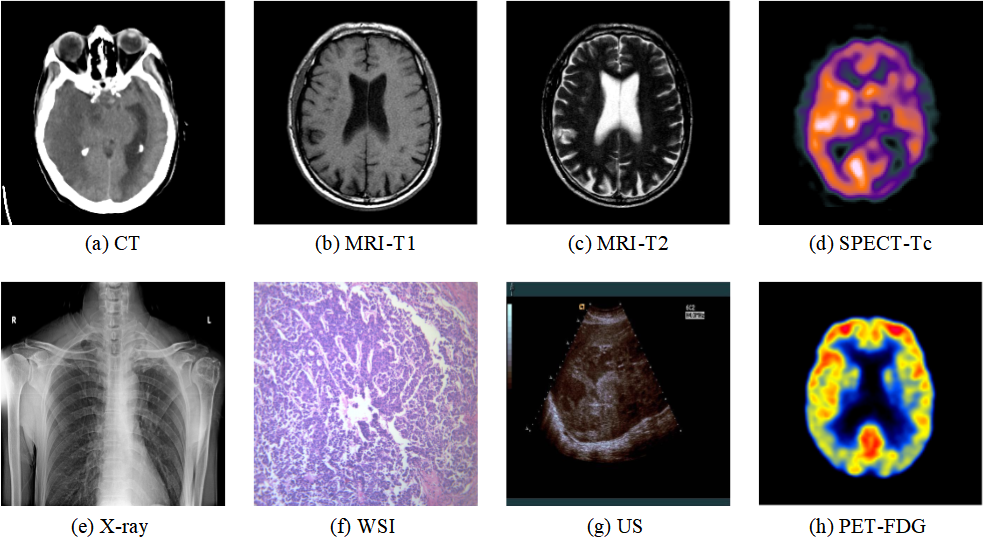
\includegraphics[width=0.9\linewidth]{figs/mul_imaging.png}
      \caption{七种不同类型的医学影像}\label{mul_imaging}
    \end{figure*}

\subsection{基于解剖结构的成像技术}
\textbf{计算机断层扫描}(CT)\cite{boyd1983cardiac}是一项以X射线成像为基础的医学影像技术,通过对人体特定部位进行X射线扫描,利用探测器接收透过人体的X射线并转换为电信号,最终生成数字化的横断面影像。其工作原理包括X射线透过人体产生的信息采集、数字影像处理和影像重建。
CT影像的构建涉及到对扫描区域的体素进行X射线吸收系数或衰减系数的测量,这些数据通过计算机处理后形成数字矩阵,再转换为灰度影像。影像的空间分辨力取决于像素大小和数目,CT影像的像素通常为1.0 × 1.0 mm或0.5 × 0.5 mm,数目可达256 × 256或512 × 512,因此,CT能够提供高度细致的解剖影像,具有较高的空间分辨力。

CT影像的特色在于其灰度表示方式,黑色代表低吸收区(低密度,如肺部含气体),白色代表高吸收区(高密度,如骨骼),而相对于传统X射线影像,CT的密度分辨力更高,能够清晰地显示组织密度差异较小的软组织结构。这使得CT在展示由软组织构成的器官(如脑、脊髓、肺等)以及病变的影像上具有突出的优势。
CT在中枢神经系统疾病的诊断上表现出色,广泛应用于颅内肿瘤、脑梗塞、脑出血、外伤性脑损伤等疾病的检测。
%螺旋CT扫描技术使其能够获得更为精细和清晰的血管重建影像,可用于CTA(CT血管成像),有望替代传统的脑血管造影
尽管CT在医学诊断领域取得了显著进展,但其使用也存在一些问题,如辐射暴露和对软组织对比度较低。随着技术的不断改进,CT仍然是一种重要的影像学工具,对于临床诊断和治疗的支持具有不可替代的作用。

\textbf{核磁共振成像}(MRI)\cite{young1984nuclear}是一种利用磁场和无线电波探测人体组织的详细横截面影像的技术。在进行磁共振成像(MRI)检查时,患者被置于一个强度高且分布均匀的静态磁场内,利用特制的无线电频率脉冲激活体内氢原子的自旋核,从而引发共振反应并捕获相应的信号。这些信号运用计算机的处理后生成高分辨率的影像,展示了人体内部的详细结构。

MRI的两种主要成像方式
%(T1、T2是用于测量电磁波的物理量,T1看结构,T2看病变)
:MRI-T1(T1反映的是纵向弛豫时间)和MRI-T2(T2反映的是横向弛豫时间),通过对比度和信号强度的不同分别对应于不同的组织特性。MRI-T1成像对脂肪组织具有较高的信号强度,呈现亮白特征,有利于显示解剖结构和脂肪组织的分布,适用于解剖结构和骨髓等的观察。相反,MRI-T2成像对水分组织有较高的信号强度,呈现亮白特征,更适用于显示水肿、炎症和软组织病变。这种高度区分不同组织的成像方式使MRI在临床上得到广泛应用,涵盖了中枢神经系统、心血管系统、关节、软组织、盆腔脏器等多个部位的病变检查。
MRI在医学影像学中的主要优势之一是对软组织的高分辨率成像。在头颅、纵隔、腹腔等实质性脏器的检查中,MRI表现出卓越的成像性能。由于人体组织成分的差异,MRI能够产生不同的信号,成为一种精准而全面的影像诊断工具。
%与传统的X线检查和核医学检查不同,MRI避免了射线辐射,因此对特定病症和人群更为安全。尽管MRI设备费用较高,对金属敏感且扫描时间较长,但在医学影像学中的不可替代作用不断凸显。

MRI技术的不断发展和创新进一步丰富了其应用领域,涵盖多种变体,如静息态磁共振成像(rsMRI)、sMRI和fMRI。每一种变体都在特定领域中展现出独特的优势。sMRI通过施加外部磁场和无线电波,激发人体组织中的氢原子核,然后测量它们在磁场中的共振信号。通过复杂的数学算法,特别是傅里叶变换,这些信号被转换成详细的影像,揭示了身体内部的精细解剖结构,为肿瘤、损伤和先天性异常等病变提供详细的解剖学信息,在神经外科和器官移植等手术前的评估中得到广泛应用。fMRI通过测量血氧水平变化,观察大脑在执行任务时的活动,提供时空分布的神经活动信息。在神经科学研究中,fMRI起到关键作用,用于研究认知功能、感觉知觉和运动执行,同时在神经精神病学和神经内科等领域用于评估神经系统疾病的功能改变。rsMRI是一项测量大脑在安静状态下血流和神经活动的成像技术。通过揭示大脑静息状态下的功能连接性,rsMRI为研究大脑的静息状态、神经网络连接性以及精神疾病、脑功能障碍等提供有益信息。这些MRI的变体在医学和研究领域中各自发挥着独特的作用,医生和研究人员可根据不同的研究和诊断需求选择适当的MRI变体,共同推动医学影像领域的不断发展,为深入理解人体生理和病理提供了丰富的信息资源,有望为未来的医学研究和诊疗提供更精准、全面的支持。

\textbf{超声成像}(US)\cite{newman1998history}是一种利用超声波对人体进行扫描的技术,它通过捕捉和分析反射回来的声波信号来构建体内器官的影像。
%其中,阵列声场延时叠加成像是超声成像领域中最传统、最简单且应用最为广泛的成像方式之一。这种方法通过对阵列的各个单元引入不同的延时,然后将它们合成为一个聚焦波束,从而实现对声场各点的清晰成像。
医学中的超声仪器涵盖了多种类型,其中B型超声是目前应用最为广泛的诊断方法。医学超声波成像是通过超声探头发出的超声波携带不同组织的回波,以构建人体内部结构的影像。
%其中A型(幅度调制型)、M型(光点扫描型)、B型(辉度调制型,即B超)、D型(基于超声多普勒原理)和C型(近似电视扫描)等是常见的。B型超声是最为广泛使用的一种成像方式,通过显示不同亮度的光点来反映接收信号的强弱,从而生成二维影像。随着技术的不断发展,还涌现出一系列新的超声技术,如灰阶显示、彩色显示、实时成像、超声全息摄影、穿透式超声成像、超声计算机断层成像、三维成像和体腔内超声成像等。
%超声诊断仪器包括A型、M型、B型、D型和彩色多普勒血流显像仪,它们各自具有独特的影像特点,其中B型超声是目前应用最为广泛的诊断方法。
医学超声波成像是通过超声探头发出的超声波携带不同组织的回波,以构建人体内部结构的影像。B模式超声影像(B超)是其中最常见的一种,其优势在于无电磁辐射、便于携带且提供实时成像。

超声诊断依赖于细致的深入观测与评估,识别不同的特征,并将这些信息整合以推断可能的病理原因。超声检查广泛应用于内脏器官的定位、测量及形态分析,同时能够帮助诊断病灶的具体范围及其性质,并提供有关腺体等组织的精确解剖影像,已在眼科、心血管以及妇产科等多个医疗领域得到普遍采用。
医生在超声检查中综合评价器官的形态、尺寸、质地、病变的声学特性、对后壁声波的影响、内部结构、位置关系及功能表现。对于不同类型的病理性影像特点,例如囊性与实质性病变、均质性与非均质性病变、钙化性与含气性病变、炎性与纤维化病变以及良性与恶性病变,医生能够通过综合观察进行诊断和鉴别诊断,为制定治疗方案提供重要参考。

\subsection{基于功能性的成像技术}
\textbf{单光子发射计算机断层成像术}(SPECT)\cite{jaszczak1980spect}是一种重要的医学成像技术,通过利用放射性同位素的$\gamma$射线,提供了对生物体内部功能和生物学过程的独特洞察。该技术基于放射性同位素的放射性衰变原理,通过测量$\gamma$光子的产生和探测,以获取有关生物体内部结构和功能的信息。
%SPECT的基本成像原理涉及患者摄入含有适当半衰期的放射性同位素药物,如锝-99m等。当这些药物到达需要成像的断层位置时,由于放射性衰变,产生$\gamma$光子。外层的$\gamma$照相机探头分布在病人周围,负责探测沿一条投影线进来的$\gamma$光子。通过闪烁体将探测到的高能$\gamma$射线转化为光信号,再通过光电倍增管将光信号转化为电信号。这些测量值代表了人体在该投影线上的放射性之和。通过多个观测角度,可以获取多个断层的平行束投影,称为平片。计算机断层成像术(CT)通过从不同角度观测,重建断层影像,将其转化为SPECT技术的重要应用。

SPECT在分辨率方面存在一些限制,如相对较低的空间分辨率和较差的时间分辨率,但其在医学影像学中的广泛应用使其成为疾病诊断和治疗方案制定的不可或缺的工具。SPECT的优势在于其提供的是功能性信息,而非仅仅是解剖结构。这对于疾病的早期诊断和治疗效果评估至关重要。如:
%心脏灌注断层显像是SPECT在心血管领域的应用的代表。它对冠心病、心肌梗死等疾病的诊断提供了支持。通过评价冠状动脉病变范围,对冠心病危险性进行分级,以及对心肌细胞活力的评估,SPECT为心血管疾病的精准诊断和治疗提供了有力工具。
在神经科学领域,局部脑血流断层显像是SPECT的一项关键应用。它对缺血性脑血管意外、癫痫致痫灶的定位等提供了高度准确的诊断。这项技术在判断脑肿瘤的血运、鉴别术后或放疗后的复发和瘢痕等方面也具有独特优势。
AD的早期诊断是SPECT在神经影像学上的又一亮点。通过对AD患者的局部脑血流进行研究,SPECT为该疾病的早期诊断提供了一致的共识。相较于传统的CT,SPECT在痴呆程度和认知状况相近的两类痴呆的鉴别上更为可靠。
%然而,SPECT的分辨率问题仍然是该技术面临的挑战之一。空间分辨率通常较低,受$\gamma$射线穿透能力和探测器灵敏度的限制。这限制了SPECT在显示小尺寸结构方面的能力。此外,时间分辨率相对较差,因为需要较长的采集时间来获取足够的数据。这使得SPECT在一些需要高时间分辨率的应用场景中受到限制。

%尽管SPECT具有一些限制,但其优势包括提供丰富的功能性信息、多模态成像、全身成像和无创性检查。它是一种非常有价值的临床工具,特别是在疾病的早期诊断和治疗方案的制定上。同时,SPECT在医学影像学中与其他技术的结合,如计算机断层成像术(CT),形成了SPECT/CT系统,为医生提供更全面的影像信息。
然而,SPECT也存在一些挑战和局限性。其中之一是辐射暴露,因为该技术需要使用放射性同位素。尽管通常在安全范围内,但这仍然是需要考虑的问题。此外,SPECT的设备和维护成本相对较高,这可能限制其在某些医疗机构的推广和应用。同时,SPECT依赖放射性同位素的摄入,这可能涉及到一些限制和患者安全的问题。
%综合而言,SPECT作为一种功能性成像技术,在医学影像学中发挥着重要作用。尽管其分辨率方面存在一些限制,但其在疾病的早期诊断、病理学分析和治疗方案制定方面提供了重要的支持。随着技术的不断发展,SPECT在医学领域的地位有望不断提升,为更准确的疾病诊断和治疗提供更多可能性。

    
\textbf{正电子发射断层成像术}(PET)\cite{raichle1983positron}作为一种核医学成像手段,它依赖于正电子在湮灭过程中释放的辐射光子。在这个过程中,回旋加速器将带电粒子加速,并轰击特定的靶核,进而生成正电子放射性核素。通过精心设计的探测器阵列和高效的符合电路,PET能够检测到这些湮灭光子对,并据此绘制出体内正电子核素的截面分布图。这种影像能够清晰地展示病变的位置、形状、大小,以及相关的代谢功能,为医生提供宝贵的诊断信息。
%尽管PET存在辐射剂量较大和设备成本高的缺点,但其独特优势在于提供高分辨率的功能性信息,广泛应用于肿瘤学、心血管学等领域,为疾病的早期诊断和治疗效果评估提供重要支持。

在肿瘤学中,PET成像被广泛用于癌症的早期诊断、分期、治疗效果评估和复发监测。18F-FDG(2-氟-18-氟-2-脱氧-D-葡萄糖)是一种常用的显像剂,通过显示异常的葡萄糖代谢水平,PET可以精准定位和描绘肿瘤。在实际应用中,患者接受18F-FDG药物注射后,PET扫描仪通过探测正电子湮灭事件获取体内放射性核素分布情况。影像分析利用标准化摄取值(SUV)等定量测量,对病变的代谢活性进行评估,为肿瘤生物学特性、治疗反应和复发监测提供关键信息。

%在心血管学中,PET可评估心肌的代谢和灌注情况,用于诊断和监测冠心病、心肌梗死等疾病。正电子放射性核素的注射提供心肌代谢信息,例如18F-FDG PET用于评估心肌葡萄糖代谢。此外,PET与CT结合可提供更全面的心血管影像信息,为精准诊断和治疗规划提供支持。

在神经学领域,18F-FDG PET在AD早期诊断中取得显著进展。通过评估脑部葡萄糖代谢情况,PET揭示患者大脑功能异常,为AD的诊断和病程监测提供关键信息。 PET的高分辨率和功能性信息使其在医学中的应用不断拓展,为多领域的疾病管理提供了更全面、精准的影像学支持。

\subsection{基于其他类型的成像技术}
\textbf{X射线}(X-ray)\cite{warren1990x}是一种电磁辐射,在医学影像学中,X射线被广泛用于探测和成像,广泛用于识别骨骼问题、胸部及腹部疾病,包括肺部与肠道堵塞等状况。X射线成像主要依赖于光电效应,通过测量透射或散射的X射线来获取关于人体内部结构的信息。
%X射线的分辨率取决于成像设备的性能,现代X射线设备通常能够提供较高的分辨率,能够清晰地显示细小的解剖结构。X射线的成像机制是通过穿透物体并被探测器接收,形成影像。这使得医生能够检查骨骼、器官和其他组织的内部结构,帮助做出准确的诊断。然而,对于柔软组织和微小病变的检测,X射线的分辨率相对较低,有时需要进一步的影像检查或其他影像技术的辅助。

%X射线成像的原理是通过X射线的吸收和散射来区分不同组织的密度和构造。当X射线经过人体时,不同组织对X射线的吸收能力不同,因此在胶片或数字探测器上形成不同的灰度影像。这些影像可以由医生进行解读,从而进行疾病的诊断和评估。
X射线成像的优点之一是其广泛的应用范围和相对较低的成本。X射线设备相对便宜且易于使用,使得它在许多医疗机构中得到了广泛的普及。此外,X射线成像速度快,可以提供即时的影像结果,对急诊情况和危重患者的救治具有重要意义。
然而,X射线成像也存在一些缺点和风险。首先,X射线是一种电离辐射,长期频繁暴露可能对人体产生辐射损伤的风险,特别是对于儿童和孕妇。其次,X射线成像对柔软组织的分辨率较低,不适合检测早期病变或微小的异常。

%综上所述,X射线成像具有快速、广泛应用和相对低成本的优点,但也存在辐射风险和对柔软组织分辨能力有限的缺点。在实际应用中,医生会根据患者的具体情况和病情选择合适的影像技术来进行诊断和评估。

\textbf{显微镜}\cite{haider1998electron}作为一种基于凸透镜成像的仪器,在医学中发挥着广泛的作用。通过物镜和目镜的双重放大过程,显微镜能够将微小物体放大到人眼可分辨的尺寸,为医学研究提供了重要的支持。
%其主要组成部分包括目镜、物镜、载物台和反光镜,其中物镜的焦距小于目镜,而反光镜用于反射光线,照亮被观察的物体。
在医学领域,显微镜的应用涉及组织学、细胞学和病理学等多个方面。通过观察组织切片(whole slide image,WSI),显微镜可以提供高分辨率的影像,帮助医生深入了解微观结构,从而支持准确的疾病诊断和治疗方案的制定。

特别是在癌症研究和诊断领域,显微成像技术发挥着至关重要的作用。如:
%显微成像可用于深入研究癌症组织的结构和形态学特征。通过对组织切片的显微观察,医生能够详细了解癌细胞的外观、大小、核形态等信息,有助于明确肿瘤类型。另外,
显微镜下的成像可用于对癌症病理学进行详细分析,包括观察组织的完整性、细胞浸润深度以及细胞变化的程度。这些信息对于判断肿瘤的恶性程度至关重要。尽管显微镜具有高分辨率、实时观察和非侵入性等优点,但也存在一些挑战,如有限的穿透深度、专业训练要求和较高的设备成本。
近年来,随着技术的不断创新,显微成像在医学领域的应用前景将继续扩展。新兴技术如活体显微镜技术使得在活体动物或人体上进行实时显微观察成为可能,为研究疾病的生长过程、细胞动态和治疗效果提供了更为深入的理解。
%总体而言,显微成像技术在医学研究中发挥着不可替代的作用,为深入了解疾病机制和制定更精准的治疗方案提供了强大的工具。
   \begin{table*}[htbp]
      \centering
      \small
          \caption{不同的医学影像成像机制、分辨率及优缺点对比}\label{imaging_contrast}     
            \begin{tabular}{cccm{2.7cm}<{\centering}m{2.7cm}<{\centering}}
            \hline
            \textbf{\textit{Imaging}} &成像机制 &分辨率 &优势 &局限性  \\ \hline
            \textbf{X-ray} &X射线 &[0.1mm,~1mm]  &成像速度快、价格低、广泛应用  &X射线有害、软组织成像效果差  \\ \\
            \textbf{CT}	&X射线  &[0.5mm,~2mm]  &成像速度快、价格低、骨组织敏感  &X射线有害、软组织成像效果差、有伪影  \\ \\
            \textbf{MRI} &磁共振  &[0.5mm,~1.7mm]  &软组织成像效果好、无骨伪影  &硬组织成像效果差、时间较长  \\ \\
            \textbf{US}  &超声波  &[1.5mm,~2mm]  &成本低、无损耗、使用方便  &分辨率较低、无法穿透骨骼、空气、存在折射效应  \\ \\
            \textbf{SPECT} &$\gamma$射线  &[3.5mm,~10mm]  &对比度高、提供功能性信息、价格较低  &分辨率较低、速度慢、放射性同位素的摄入  \\ \\
            \textbf{PET} &核  &[4mm,~6mm]  &高分辨率、提供功能性信息  &放射性同位素的摄入、成本较高  \\ \\
            \textbf{WSI} &凸透镜  &[200nm,~0.2$\mu$m]  &高分辨率、实时观察、非侵入性  &有限穿透深度、需要专业训练、成本较高  \\  \hline
            \end{tabular} 
    \end{table*}


不同的成像机制可以获得不同的医学影像,并根据不同的特性应用于不同的疾病诊断中,各自的特性比较如表\ref{imaging_contrast}所示,表中的分辨率通常在给出的参考范围内,具体值取决于设备的类型和扫描参数等使用的条件。X-ray主要用于颅骨成像,对于骨折和骨质疾病的检测具有优势。CT提供高分辨率的骨髓和软组织影像,对脑肿瘤的大小和位置具有关键意义。MRI适用于探测脑部软组织病变,如脑肿瘤、AD等。US在产前检查和婴儿脑部检查方面有优势。SPECT在AD早期诊断方面有帮助,而PET在脑肿瘤代谢活性和AD脑代谢方面表现出色。显微成像对神经系统疾病的基础研究和理解细胞水平变化至关重要。在实际应用中,这些成像技术的综合运用可以更全面地观察和诊断疾病。
%例如,X射线和CT适用于颅骨骨折检测,MRI用于详细结构描绘脑肿瘤,SPECT和PET提供关于脑功能和代谢的信息,显微成像则助力深入理解神经系统疾病的微观变化。

在医学影像领域,倘若有一台能够扫描多模态的医学影像数据的机器会极大地提高诊断效率和准确性。然而,由于成本和设备更新的限制,在国内医疗环境中,许多医院只拥有特定类型的扫描仪,其产生的影像局限于该仪器的特性。这就迫使医生必须根据需要使用不同的设备,增加了工作的复杂性。若有一种简便且高效的算法,能够将来自不同设备的影像进行融合,将为医学影像的多模态融合提供一种经济高效的解决方案。
因此,开发出能够实现多模态融合的算法,不仅能够在医学影像的全面性诊断上大显身手,同时也能为医院节省设备购置成本和提高工作效率。这种简单而实用的技术创新,无疑将为医学领域带来福音。



\section{智能影像组学技术的理论基础}


\subsection{医学影像组学关键技术介绍}
%随着人工智能技术的迅猛发展,涌现出许多分类模型,主要分为基于传统的机器学习(Machine Learning,ML)方法和基于深度学习(Deep Learning,DL)方法两大类别。这些分类模型在医学领域的应用正不断扩展和深化,涵盖了诸如肿瘤检测、疾病诊断、影像分割等多个方面。它们不仅提高了医学影像分析的效率,同时为医疗诊断带来了更准确的结果。在医学科研和临床实践中,这些模型的不断进步为提升医学影像技术水平和改善患者医疗体验贡献了重要力量。
医学影像组学是一个交叉学科领域,它结合了医学影像学、生物信息学、计算机科学和数据科学等多个学科的知识和技术。在过去,医学影像组学的分析往往依赖于传统的手工设计特征,即研究者根据以往的经验和知识来选择和定义特征。在智能辅助诊断方面,最初主要依赖于基于机器学习的方法,这些方法通常需要人工设计特征,即研究者需要根据专业知识来选择或构造用于模型训练的特征。然而,近年来深度学习技术的兴起和发展,使得医学影像组学能够通过神经网络来自动学习和提取特征,这一变革减少了对专家知识的依赖,显著提高了特征提取的效率和准确性。

\subsubsection{基于传统的机器学习方法}
基于传统的ML方法,如支持向量机(SVM)、决策树、随机森林等,以其稳定性和可解释性在医学影像分类任务中取得了显著的成果。%这些方法通过提取手工设计的特征,对医学影像进行分类和识别,为医学诊断提供了一种可靠的解决方案。
本章将多种常见的ML方法进行比较,见表\ref{ML_contrast},并详细分析经典的SVM分类器。

   \begin{table*}[htbp]
      \centering
          \caption{常见的基于传统的机器学习方法对比}\label{ML_contrast}     
            \begin{tabular}{m{3.2cm}<{\centering}m{4.2cm}<{\centering}m{4.2cm}<{\centering}}
            \hline
            \textbf{\textit{ML方法}}  &优势 &局限性  \\ \hline
            \textbf{支持向量机}  &SVM模型只与支持向量有关、高维数据中只需少量的样本、节省了内存,鲁棒性强  &非线性SVM需要进行核函数映射、计算开销较大  \\ \\
            \textbf{贝叶斯}	  &实现简单、收敛速度快、聚类效果较优、无参数训练模型  &k需要人为设定、只能得到局部最优解、抗干扰差、非凸数据集难以收敛  \\ \\
            \textbf{决策树}  &对数据要求度低、速度快、准确性高、适合高维数据  &在训练数据上比较耗时、在面对复杂的高维数据时容易过拟合  \\ \\
            \textbf{随机森林}    &实现简单、准确性较高、适合高维数据  &整组数据的决策树上容易过拟合、训练时间较长  \\ \\
            \textbf{逻辑回归} &计算速度快、适合二分类、内存占用小、模型可解释性好  &不能解决非线性问题、很难处理数据不平衡的问题、准确率不高  \\ \\ 
            \textbf{K-最近邻} &实现简单、可直接在测试数据上查找最近的邻居来进行分类 &依赖于距离度量、计算成本高、不适用于高维稀疏数据
             \\  \hline
            \end{tabular} 
    \end{table*}
    
   \begin{figure*}[htbp]
      \centering  
      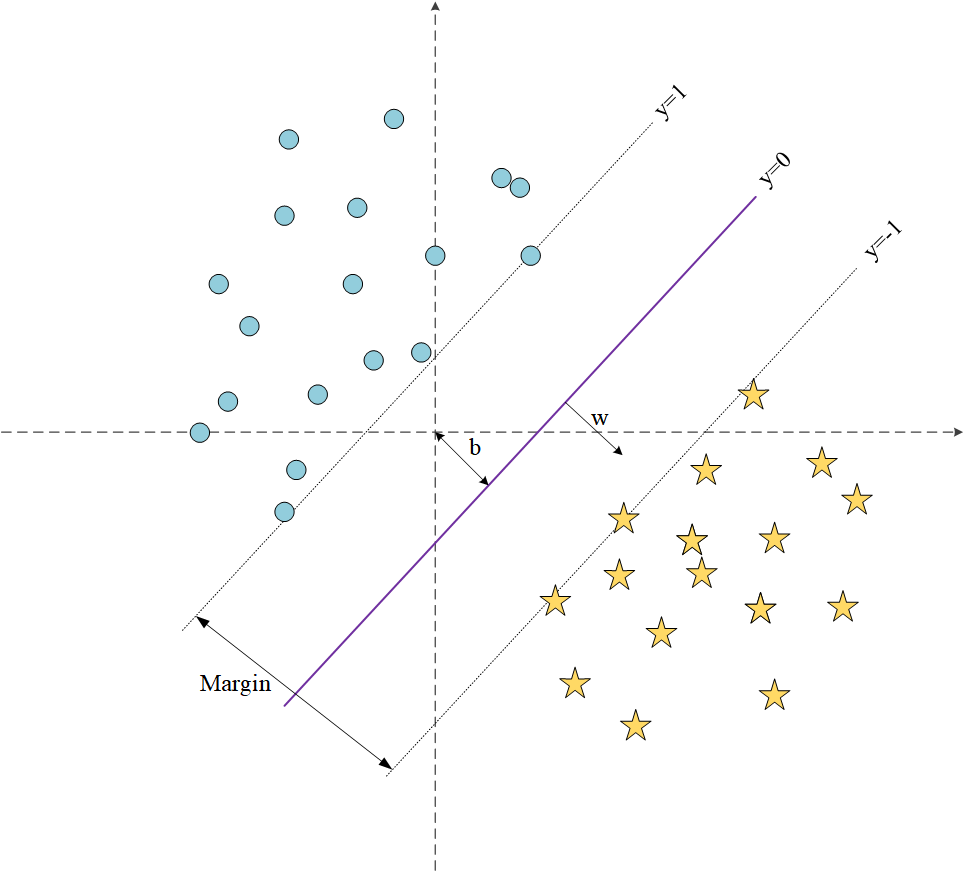
\includegraphics[width=0.9\linewidth]{figs/svm.png}
      \caption{线性可分SVM}\label{svm}
    \end{figure*}
    
在二分类模型中,支持向量机(SVM)是一种广泛应用的方法。其核心分类思想是寻找一个能够将样本分割并具有最大间隔的超平面。这里的“间隔最大”指的是确保超平面与其最近的样本点的距离最大。通过最大化间隔,SVM能够提高分类预测的可信度。如图\ref{svm},中间的实线即为所求的最优超平面,虚线边界上的点被定义为支持向量。最优超平面到两侧虚线边界的距离是相同的,这个距离称为几何间隔,Margin即为两倍的几何间隔,其计算为$2/\|\mathbf{w}||$。y是分类面,其计算为$\text{wx+b}$。线性可分SVM可归为凸二次规划问题,针对该类问题可以考虑用Lagrange乘子法进行求解,目标函数为公式(\ref{SVMst})。
\begin{equation}\label{SVMst}
\begin{aligned}\min\frac{1}{2}\|W\|^2\\\\s.t.\quad y_i\left(W^Tx_i+b\right)\geq\pm1\end{aligned}
\end{equation}

线性可分SVM在面对非线性可分的样本集时显然存在局限性。为了解决这一问题,SVM采用了核函数$\phi(x)$的方法,典型的核函数包括RBF(径向基函数),poly(多项式核函数),linear(线性核函数),sigmoid等。SVM使用这些核方法把数据映射到高维,以便更好地分离。具体而言,非线性可分SVM的模型可以表示为式(\ref{svm2}):
\begin{equation}\label{svm2}
f(x)=W^{T}\phi(x)+b
\end{equation}

其中,$\phi(x)$表示样本在高维空间中的映射,$W$是对应的权重向量,$b$是偏置项。通过这样的映射,原本在低维空间中无法线性分隔的样本,在高维空间中找到了一个线性超平面,从而完成了分类任务。这种非线性可分SVM的处理方式为算法赋予了更大的灵活性,使其能够更好地适应实际场景中存在复杂结构和非线性关系的数据。
%在医学领域,特别是医学影像分类与预测任务中,这种能够处理非线性关系的SVM模型为提高准确性和适用性提供了有力的工具,有助于更精准地识别和预测医学影像中的复杂模式。在多分类问题中,支持向量机(SVM)采用直接法和间接法两种构建策略。直接法通过修改目标函数解决多个超平面参数的最优化问题,适用于小型数据集但计算复杂度较高。间接法基于多个二分类器构建多分类器,有“一对一”和“一对其余”两种实现方式,前者需要设计 $k(k-1)/2$个分类器,后者则设计K个分类器。在实际应用中,选择适当的构建策略需考虑数据集规模、计算资源和对模型解释性的需求,这对于获得更好的性能至关重要。

SVM作为一个多才多艺的分类器,不仅在ML领域取得了成功,而且在医学影像处理中表现出色,为医学领域的疾病诊断和预测提供了强大的支持。其能够同时应对线性和非线性的分类任务,为医学影像的自动化分析和医生的决策提供了可靠的辅助。
%尽管SVM在医学影像处理中具有许多优点,包括高准确性和泛化能力,但在处理大规模数据、调整核函数参数以及对噪声和异常值的敏感性等方面仍然存在一些挑战。在实际应用中,需要仔细权衡其优势和缺陷,并结合具体问题的特点选择适当的算法。

\subsubsection{基于前沿的深度学习方法}
基于DL方法的发展更是推动了医学影像处理的前沿。卷积神经网络(CNN)和循环神经网络(RNN)等深度学习架构通过学习影像的高级特征表达,使得模型能够自动从数据中学习到更抽象、更复杂的表示,从而在医学影像分类中取得了卓越的性能。DL方法的主要优势在于其端到端的学习能力,对于复杂和大规模数据集的处理能力更为突出。

   \begin{figure*}[htbp]
      \centering  
      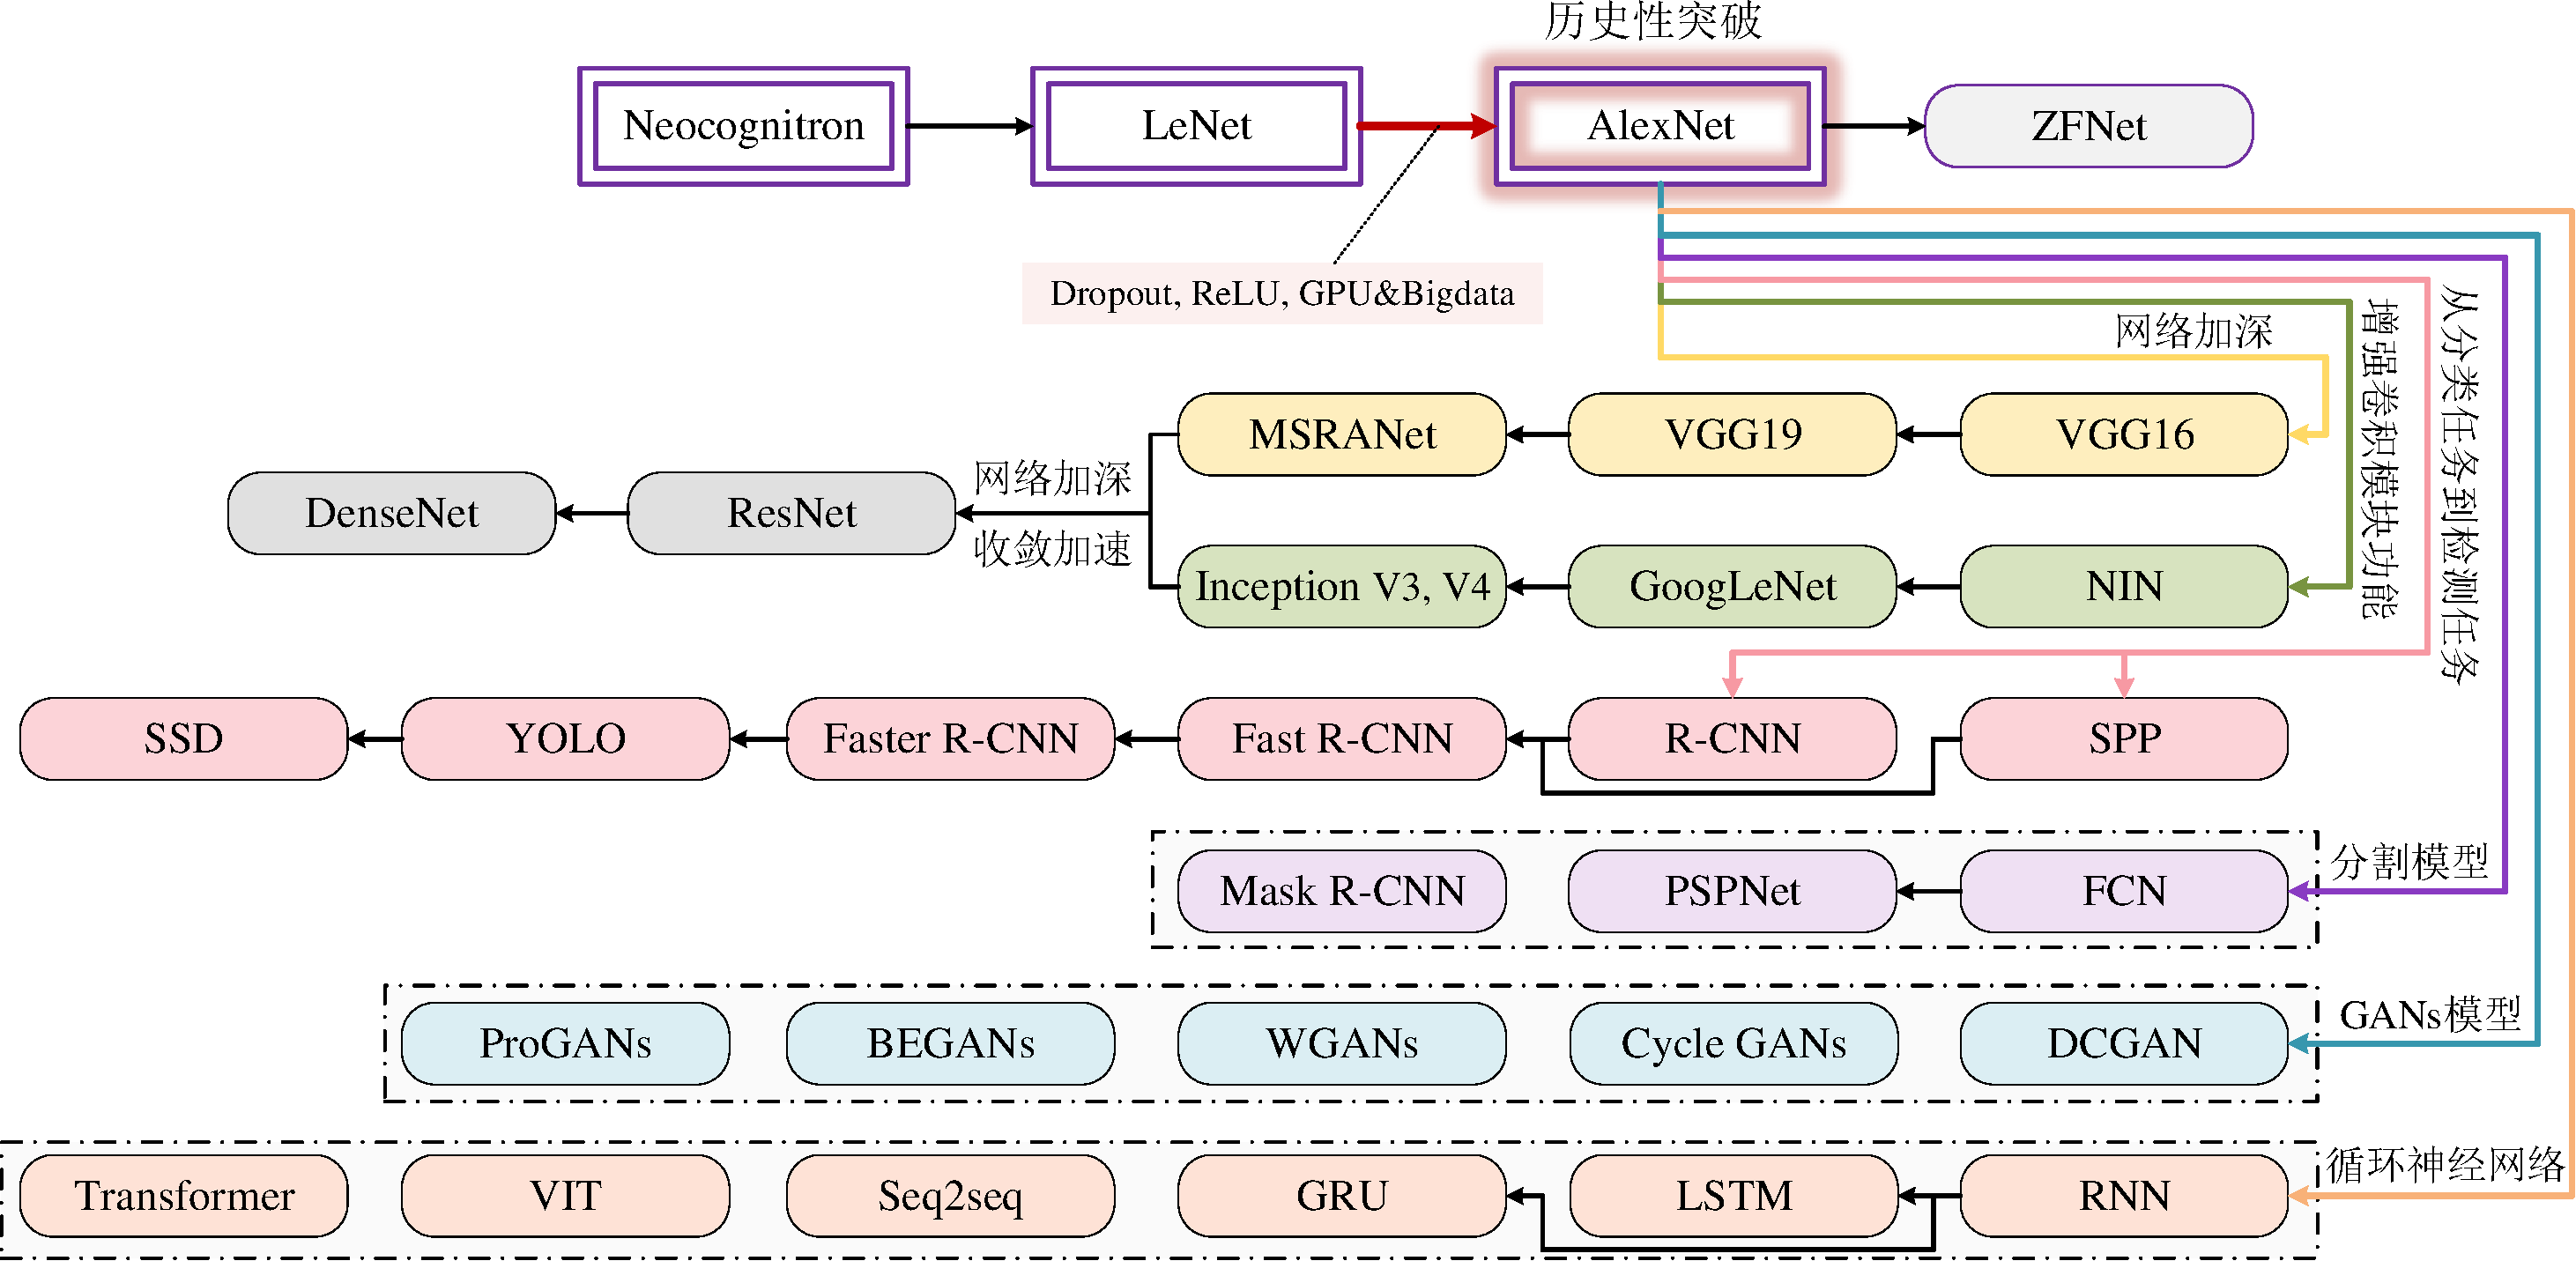
\includegraphics[width=0.9\linewidth]{figs/CNNdevelopment.pdf}
      \caption{深度神经网络发展脉络}\label{CNNdevelopment}
    \end{figure*}
    
CNN代表了DL领域的重要里程碑,其模拟了生物神经元结构的并行计算方式,能够在分类任务中自动学习和提取数据中的抽象特征,从而无需依赖手工设计的特征。CNN相对于传统机器学习方法在影像融合、分类、预测等任务中具有显著优势。其核心技术包括卷积、激活、批归一化、池化和全连接。
在影像分类领域,CNN通过卷积操作实现对输入影像的特征提取,利用局部感知和权值共享机制捕捉影像的局部特征,使得模型能够更好地适应数据的复杂结构。激活函数引入非线性,如Sigmoid、Tanh、Softmax和ReLU,赋予模型对复杂关系的学习能力。批归一化在神经网络的中间层中规范输入,加速训练过程,提高模型的稳定性。池化操作通过降采样减小特征图的尺寸,有助于保留重要信息并降低计算复杂度。全连接层整合局部特征,并将其映射到样本标签空间,完成最终分类。

    
CNN在实际应用中展现出卓越的性能,尤其在计算机视觉领域,为处理庞大而复杂的数据集提供了高效而强大的解决方案。图\ref{CNNdevelopment}为CNN的大致发展脉络。其中,LeNet\cite{lecun1998gradient}作为CNN的经典之作,为DL领域的发展奠定了坚实基础,成为影像分类和识别领域的开创性工作。AlexNet\cite{krizhevsky2012imagenet}在某种程度上继承并发展了LeNet的思想,并且引入了一些新的技术,如在CNN中广泛使用了ReLU激活函数,使用了Dropout技术防止过拟合,并采用了GPU加速训练过程。AlexNet的模型结构如图\ref{Alexnet}所示,它在2012年的ImageNet大规模视觉挑战赛
%(ImageNet Large Scale Visual Recognition Competition,ILSVRC)
中取得了冠军,其不仅在性能上大幅超越了当时的其他方法,而且其成功也证明了DL在处理大规模视觉识别任务中的巨大潜力,极大地促进了DL在各个领域的应用和发展。 

AlexNet等CNN网络模型在医学领域的应用为医学影像分析、疾病诊断和个性化医疗等方面带来了巨大的进步,推动了医学影像组学分析技术的发展,为医学诊断和治疗提供了全新的思路和工具。
一些经典的网络模型在医学领域取得了显著的成果,如FCN\cite{long2015fully}作为一种专门用于影像分割的模型,特别适用于医学影像的病灶分割等任务。
U-Net\cite{ronneberger2015u}是一种用于生物医学影像分割的经典网络模型,结构简单,同时在分割任务中表现出色。因此,医学领域广泛采纳并应用了这项技术。
总的来说,CNN网络模型在医学领域的应用为医疗诊断、疾病预测和治疗方案的制定带来了更多的可能性和机会,有助于提高医疗保健的水平和效率。

 \if 0
   \begin{figure*}[htbp]
      \centering  
      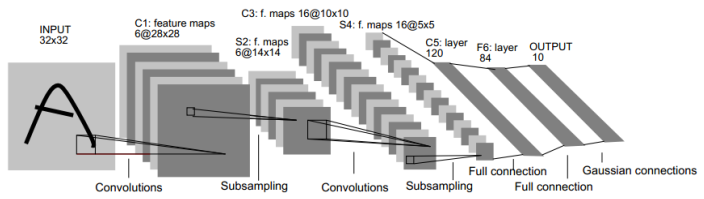
\includegraphics[width=0.9\linewidth]{figs/Lenet.png}
      \caption{Lenet网络结构}\label{Lenet}
    \end{figure*}
  \fi

   \begin{figure*}[htbp]
      \centering  
      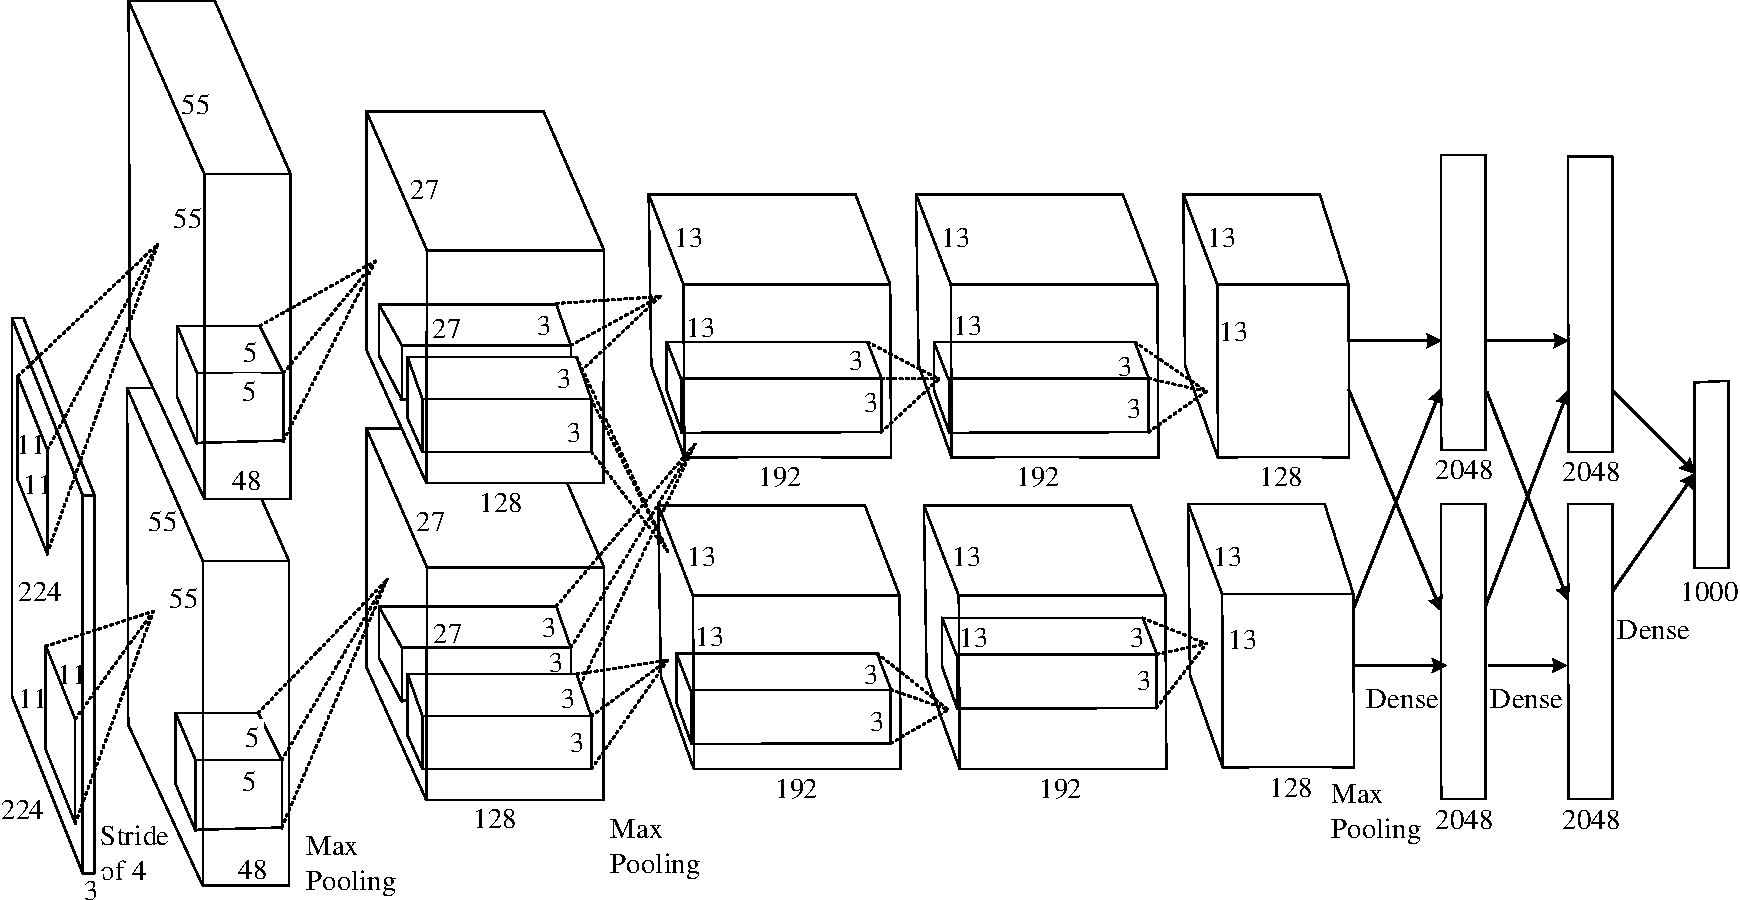
\includegraphics[width=0.9\linewidth]{figs/alexnet.pdf}
      \caption{AlexNet\cite{krizhevsky2012imagenet}网络结构}\label{Alexnet}
    \end{figure*}
%LeNet是LeCun等科学家于1998年提出的CNN模型,最初应用于手写数字和英文字母的识别任务\cite{lecun1998gradient}。该模型结构如图\ref{Lenet}所示,其包括7个层次,其中包括3个卷积层、2个池化层和2个全连接层。LeNet的输入影像尺寸为32x32,虽然规模较小,但其各个模块的设计十分完备,为后续深度学习模型的发展奠定了基础,被认为是CNN的基石之一。LeNet的结构设计反映了卷积神经网络的基本原理,通过卷积和池化层逐渐提取影像的层次化特征,最终通过全连接层进行分类。LeNet的成功证明了CNN在处理视觉任务上的有效性,为后续深度学习研究和应用的发展打下了坚实基础。


%医学领域对影像技术的需求不断增长,这两种类型的分类模型都在不同的场景中展现了强大的潜力。传统方法在数据较为有限或需要解释性强的情况下具备优势,而深度学习方法则在处理大规模数据和复杂特征提取方面取得了显著的成就。因此,这两者的结合和并行应用成为医学影像分类领域的一个前沿趋势,为更准确、高效的医学诊断提供了新的可能性。

\subsection{影像组学技术的信息融合策略}
信息融合涵盖了不同医学影像之间的融合(多模态融合),例如CT与SPECT的融合、CT与MRI的融合、MRI与SPECT的融合甚至是三种影像的融合。同时也包括影像和其他异构数据之间的融合(跨模态融合),如临床指标与医学影像之间的融合。作为一种关键的影像处理策略,尤其在多模态医学影像领域,影像信息融合通过综合多种影像信息并采取相应的融合策略,可以显著提高影像的质量和信息量。常见的融合方法主要分为三种:像素级、特征级以及决策级融合。

这三种融合方法在多模态影像融合、AD分类和PD预测的研究中备受关注。在多模态影像融合方面,这些方法为整合不同成像模态提供了高效手段,有助于充分利用各种影像信息,提高影像的全面性和信息量。在AD分类和PD疾病预测领域,融合方法的应用为更准确、可靠的疾病诊断和预测提供了新的思路和工具。通过综合不同模态的信息,可以更全面地了解患者的病理状态,为个性化治疗和康复提供更为精准的支持。这些研究不仅推动了医学影像处理技术的进步,也在提升脑部疾病的辅助诊断水平方面取得了显著的研究成果。

\subsubsection{基于像素级的技术方案}
像素级融合技术涉及在影像处理的基础层面上,对原始影像数据的像素点进行直接操作和整合,形成新的像素值,进而生成融合影像。这一方法在影像信息融合中起到重要作用,特别是在像PET和MRI影像的融合中。像素级融合技术能够有效地结合不同影像源的信息,从而增强影像细节,这有助于提升疾病诊断的准确性。将PET-MRI影像对采取像素级融合可以充分发挥PET在发现受试者脑部葡萄糖代谢变化方面的优势,尤其在AD患者中,PET可揭示脑部葡萄糖摄取降低、导致脑萎缩的情况。虽然PET影像本身的细微解剖结构分辨率不甚理想,但通过与MRI技术的联合应用,能够显著提升影像的整体清晰度和细节丰富度。二者的融合可以克服各自的局限性,为痴呆患者的病程分析提供更全面的信息。通过综合PET和MRI的数据,可以更准确地评估AD患者的病变程度,为医生提供更为精确的诊断和治疗决策支持。因此,像素级影像融合在神经学领域中的应用有望在脑部疾病的诊断和治疗方面发挥关键作用。

   \begin{figure*}[htbp]
      \centering  
      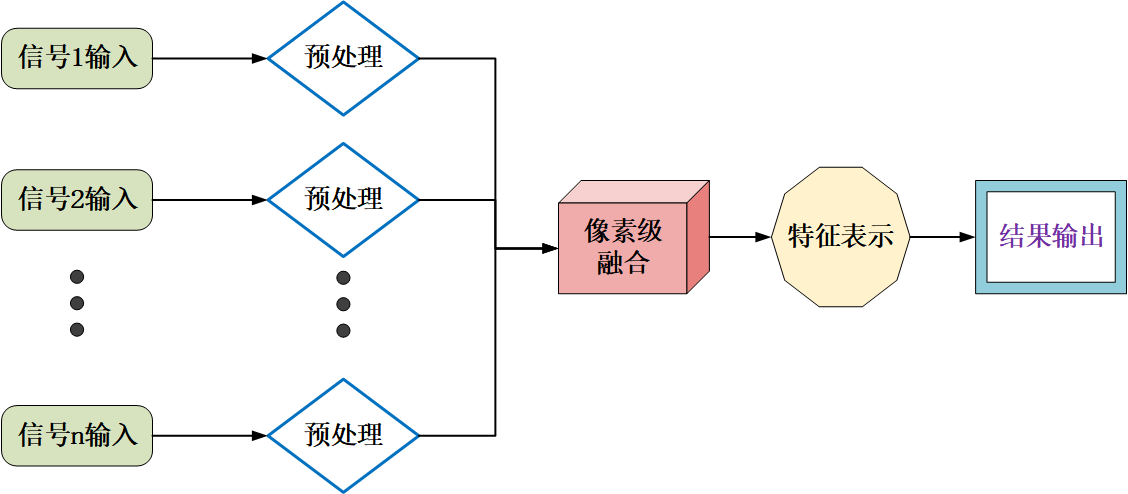
\includegraphics[width=0.9\linewidth]{figs/pixelFusion.png}
      \caption{像素级信息融合机制}\label{pixelFusion}
    \end{figure*}
    
如图\ref{pixelFusion}所示,像素级影像融合通过各类不同和类型的输入数据执行预处理操作,并采用特定的计算策略计算新的像素点数值,最终生成融合影像。这种融合策略有效地整合了来自不同来源的信息,引入更加细致的信息,并强化了影像的相关特征,具备高度的精度。像素层面的影像融合的独特之处在于能够最大限度地保留源影像中的内容,使得融合后的影像内容和细节都得到了增强。该方法有助于突显潜在目标,判断和识别潜在目标的像素点,为影像的理解和分析处理提供有力支持。

尽管像素级影像信息融合具有显著的优势,但也面临一些局限性。首先,由于像素级融合涉及大量数据的计算处理,可能导致较长的处理时间,实现实时处理与显示是一项挑战;其次,由于数据量庞大,在通信传输过程中,此类信息更易受到噪声影响。此外,如果参与融合的源影像没有经过精准配准处理,则融合后的影像可能出现模糊不清、目标定位不准确以及细节信息失真的问题。

\subsubsection{基于特征级的技术方案}
特征级影像融合通过先对不同模态原始数据进行预处理,接着运用各类模型提取各自特有的信息特征,再依据特定融合规则,将这些各异模态数据的特征有效整合起来,如图\ref{featureFusion}所示。
%以CT和MRI两种不同模态的数据为例,该融合方法首先对这两种不同模态的数据进行预处理,然后利用不同或相同的网络模型提取CT或MRI影像的特征,最后利用融合后的特征进行输出。特征级影像融合的独特之处在于能够包含不同模态影像的特征之间的相关性和交互信息,从而融合更多信息,获取更具判别力的特征表示。这种融合方法有助于综合不同模态的信息,提高对复杂目标的识别能力。
通过深度学习等技术,特征层面的影像融合技术可以自动学习并提取不同模态的有重要信息的特征,从而更好地揭示目标的多方面信息。这对于医学影像处理领域尤为关键,例如在神经影像学中,结合CT和MRI的特征级融合有助于更全面地理解脑部结构和病变。

   \begin{figure*}[htbp]
      \centering  
      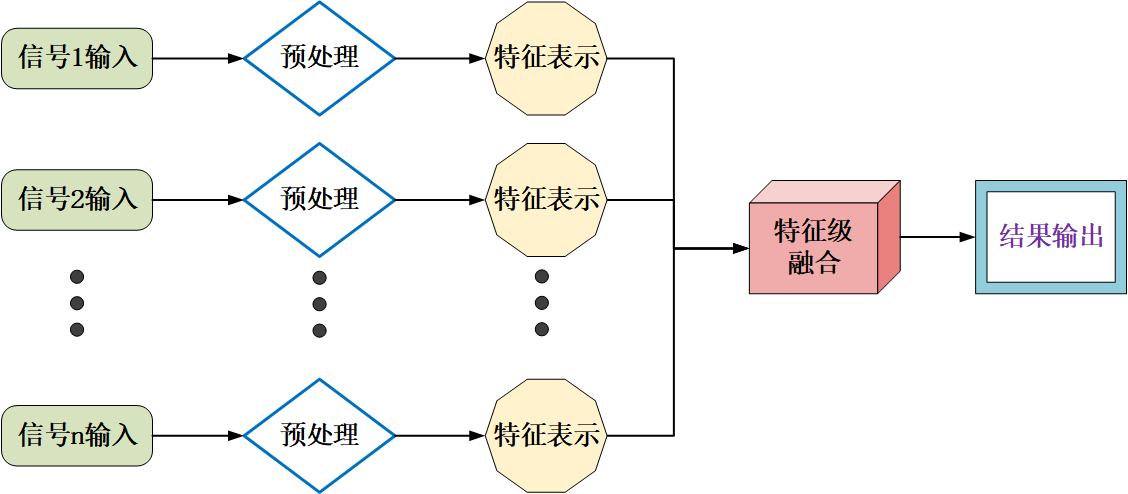
\includegraphics[width=0.9\linewidth]{figs/featureFusion.png}
      \caption{特征级信息融合机制}\label{featureFusion}
    \end{figure*}

从源影像中提取特征通常指的是识别和量化影像中的关键信息,这既包括整个影像的全局特征,也包括特定区域的局部特征(如感兴趣区域,即ROI)。例如,在医学成像领域,MRI和CT影像的特征提取旨在识别出有助于诊断的关键信息,并将这些信息进行分析和处理,以便用于后续的影像融合。通过这种方法,可以从MRI和CT影像中提取出有用的特征,然后将这些特征结合起来,形成一个更为全面的特征表示。这种特征级的影像融合方法能够有效地减少数据的冗余,提高信息的密度,从而在分类和其他影像处理任务中达到更高的准确度。相比于直接在像素级别进行融合,特征融合能够显著降低所需的计算资源和存储空间,因为它只关注影像中的重要信息,而不是每一个单独的像素。同时,特征级融合的计算速度较快,虽然对影像匹配精确度的要求相对较低。这种方法为在医学影像处理领域提供了更高效的影像信息融合策略。相比于其他方法,特征级影像融合在内存和时间上的需求较低,因此,其具有更迅速的计算效能,并能够有效提升影像处理的实时响应能力。但也可能损失部分细节性特征。

   \begin{figure*}[htbp]
      \centering  
      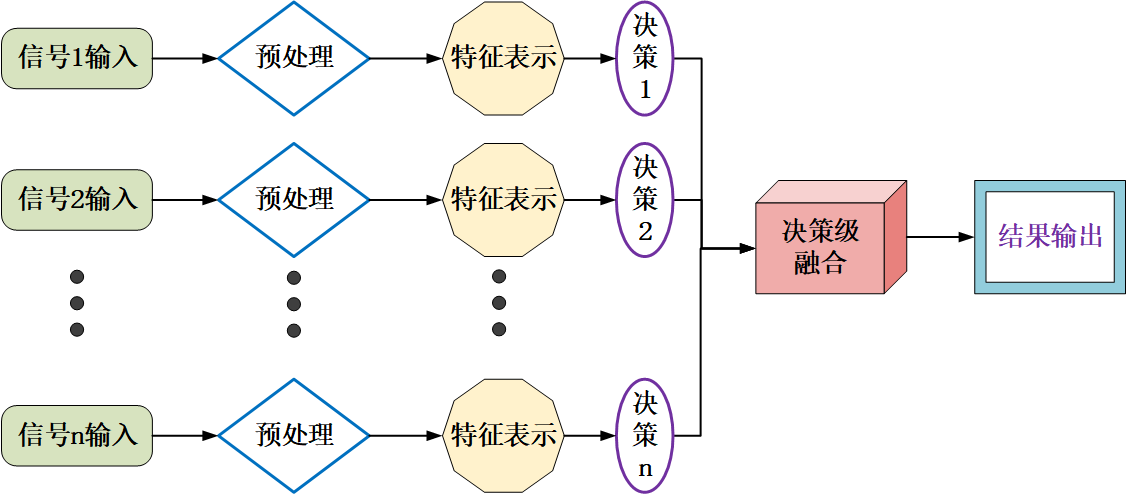
\includegraphics[width=0.9\linewidth]{figs/decisionFusion.png}
      \caption{决策级信息融合机制}\label{decisionFusion}
    \end{figure*}
\subsubsection{基于决策级的技术方案}
决策级影像融合技术被视为一种高层次的认知整合策略,它代表了影像融合技术中最复杂与最抽象的手段。此方法先将每幅影像依据各自的特征信息进行独立识别与分类处理,然后结合每个源影像的决策结果,按照一定的规则和置信度权重,如采用贝叶斯推理或是集合决策机制等,对这些决策结果进行综合集成,从而得出最优的整体判断。以SPECT和CT影像为例,在这一层级上,首先分别对两种不同模态的数据完成独立的诊断决策,随后遵循特定准则,将这两种影像的决策输出相结合,目的是为了实现整体最佳的诊断效果,进而准确区分AD病患的不同严重程度,该策略的实现如图\ref{decisionFusion}所示。

这种决策级影像融合方法在医学影像领域具有重要意义。通过将多个模态的独立决策结果合并,可以得到更全面、准确的诊断信息,提高对疾病状态的认知。例如,在AD的诊断中,结合SPECT和CT影像的决策结果,可以更全面地评估患者的脑部结构和功能,有助于提高对疾病的早期诊断和分级。这种影像融合方法的优势在于能够综合不同模态影像的信息,克服单一模态的局限性,为更准确的医学影像诊断提供支持。


决策层面的影像融合技术位于影像融合方法的顶层,它以认知理论为核心,针对具体问题需求实施深层次、有目的性的信息整合。该融合技术具有数据处理要求低、抗扰动稳定性强等优势。然而,与影像的像素级或特征级的策略相比,决策级影像融合存在明显的缺点。其关键挑战在于对前序步骤输出结果的高度依赖性,且对于影像集成的要求更为复杂。在影像集成的决策层,不仅要对每幅影像独立作出判断,而且还必须针对合并前的多项复杂预处理操作作出决策,这样的处理使得决策级融合的过程变得更加精细和复杂。

%在临床医学诊断中,成像参数、病人体位以及成像设备的差异可能导致成像质量受到噪声的影响,甚至引起几何畸变。为提高成像质量,预处理技术如影像去噪、影像配准和消除畸变等被广泛应用。这些方法有助于规范化影像,消除可能影响医学诊断准确性的因素。
%特征表示是对原始数据进行表达的过程,包括特征提取和特征选择。其目的是提升对数据的表达能力。目前,特征工程和表示学习是特征表示的两个主要研究方向。特征工程涉及手工处理数据,其与模型相对独立,因为模型依赖手工提取的特征进行目标预测。与之不同,表示学习是模型自主进行的学习过程,模型能够自动学习有用的特征,典型的表示学习模型包括深度学习模型、主成分分析模型和自编码器模型等。
%在信息融合最为关键的融合环节中,存在着多种多样的融合规则,常见的方法包括加法、乘法、取中位数、最大值、最小值、核函数加权等。选择适当的融合规则取决于问题的性质以及数据的特点,有效的融合规则有助于提高综合信息的准确性和可靠性。这一过程对于医学影像处理的精度和有效性至关重要,有助于为医生提供更准确的诊断信息。

%综上所述,像素级融合、特征级融合和决策级融合这三种结构紧密关联,彼此之间相辅相成。它们共同构建了一个分类框架,包括信息输入、预处理、特征表示、融合和最终输出等几个关键环节。特征提取和特征选择在这个框架中被统称为特征表示\cite{song2016two}。每个环节的性能都对整个分类框架的最终预测结果产生影响,类似于木桶原理,其中每个环节就像是构成分类框架的几块木板,框架的性能将受限于最短木板的长度。尽管有相似之处,它们在融合的层次上存在差异。在像素级融合框架中,由于融合发生较早,能够充分组合源图的细节内容,从而保留了较多的影像信息。然而,这也伴随着计算量较大和处理时间较长的缺陷。特征级融合框架中,融合过程发生在底层特征抽取之后,虽然减少了数据量,保留了大部分信息,但却增加了特征维数,可能导致部分细节内容的损失。最后,在决策级融合分类框架中,标签预测建立在每种分类结果的基础上,提供了比单一分类器更精准、更有效的性能。然而,这也伴随着增加的预测误差和风险。
%因此,采用哪种分类框架取决于具体的应用场景和需求。在实际应用中,需要根据问题的性质和可用数据的特点权衡这三种融合方法,这三者的互补性和适用性将在不同情境下发挥出更为明显的优势。

\section{智能影像组学技术的性能评估}
在智能辅助诊断应用研究中,对方法性能的评估是至关重要的一环。评估手段可以划分为基于主观判断的评估方法和依赖客观数据的评估方法两类。
主观评估通常采用主观视觉评价方法,特别适用于多模态影像融合方法的评估。这种评估方法依赖于人眼对影像质量和信息丰富度的感知,通过人工观察和比较来评估影像融合结果。主观评估的优势在于能够捕捉到人的感知差异,但缺点在于受主观因素和个体差异的影响,结果可能不够客观。

客观评估则采用一系列已有的评估指标来量化方法的性能。在多模态影像融合中,常用的客观指标包括信息熵(Entropy,EN)\cite{roberts2008assessment}、互信息(Mutual Information,MI)\cite{qu2002information}、结构相似性(Structural Similarity Index,SSIM)\cite{wang2004image}、标准差(Standard Deviation,SD)\cite{shi2005wavelet}、空间频率(Spatial Frequency,SF)\cite{eskicioglu1995image}、视觉信息保真度(Visual Information Fidelity,VIF)\cite{han2013new}等。这些指标能够从不同的角度和维度评估影像融合的效果,如影像的清晰度、对比度、保真度等。
在涉及分类或预测性能进行衡量时,通常采用的客观标准包括准确率(Accuracy,ACC)、召回率、F1分数、ROC(Area Under the ROC Curve,AUC)、均方误差(Mean Squared Error,MSE)等。这些指标直接衡量了模型在任务完成过程中的性能,为研究人员提供了客观、量化的评价标准。

通过主观和客观两种评估方法的结合,可以更全面地评价医学影像融合方法的性能,确保其在实际应用中具有良好的可靠性和准确性。这种评估方式有助于选择最适合特定医学应用场景的影像融合方法,旨在为临床医学领域研发更为精确且值得信赖的辅助诊断手段。


\subsection{客观评估手段}
\subsubsection{影像质量的分析与评估}
为了精确评价融合后影像的质量,通常采用一系列相关的影像指标来进行客观评价。这些指标涵盖了影像的不同方面,基于信息理论、影像特征、结构、和基于人类视觉感知\cite{han2013new}。以下是一些常用的客观评价指标,它们有助于全面了解影像融合结果的性能:

(1)基于信息理论的评估指标包含EN\cite{roberts2008assessment}、MI\cite{qu2002information}、FMI\cite{haghighat2011non}等。

信息熵(Entropy,EN)作为一种度量手段,可用来量化影像所包含的信息内容多少,计算公式为(\ref{EN}),其中$P(x_i)$是影像的灰度级别的概率。熵越高,影像信息越丰富\cite{roberts2008assessment}。
\begin{equation}\label{EN}
EN=-\sum_{i=1}^nP(x_i)logP(x_i)
\end{equation}

互信息(Mutual Information,MI)一种用来评估两个图像所含信息量的相互依存程度的度量,数值越大表示它们共享的信息量越丰富\cite{qu2002information}。公式(\ref{MI})定义了MI的计算方法,它涉及联合概率密度函数$p(m, n)$及其对应的边缘概率密度函数$p(m)$与$p(n)$。

\begin{equation}\label{MI}
M I(M, N)=\sum_{m \in M} \sum_{n \in N} p(m, n) \log \left(\frac{p(m, n)}{p(m) p(n)}\right)
\end{equation}

特征互信息(Feature Mutual Information,FMI)用来衡量特征间的互信息,值越高表示效果越好\cite{haghighat2011non}。其定义为(\ref{FMIf}),其中$F$表示融合影像,$A$和$B$表示源影像,$H_{F}$、$H_{A}$和$H_{B}$分别是影像$F$、$A$和$B$基于直方图的熵,$I_{FA}$和$I_{FB}$分别是融合影像$F$与源影像之间的特征信息量。
\begin{equation}\label{FMIf}
FMI_{F}^{AB}=\frac{I_{FA}}{H_{F}+H_{A}}+\frac{I_{FB}}{H_{F}+H_{B}}
\end{equation}



(2)基于影像特征的评估指标主要包括SF\cite{eskicioglu1995image}、SD\cite{shi2005wavelet}、$Q_E$\cite{piella2003new}、AG\cite{wu2005remote}、SCD\cite{Aslantas2015A}等。

标准差 (Standard Deviation,SD)衡量的是影像灰度级别的离散程度,较高的标准差代表影像对比度更强\cite{shi2005wavelet}。计算公式为(\ref{SD})。其中,$\mu$是融合影像F的均值。
\begin{equation}\label{SD}
SD=\sqrt{\dfrac{1}{H\times W}\sum_{x=1}^{H}\sum_{y=1}^{W}\left(F(x,y)-\mu\right)^{2}}
\end{equation}

边缘相关融合质量(Edge Correlation Fusion Quality,$Q_E$) 用于衡量边缘信息的融合质量,值越高越好\cite{piella2003new}。 计算公式为(\ref{QE})。其中,$X_i$和$Y_j$是两影像的像素值,$\bar{X}$和$\bar{Y}$是平均像素值。
\begin{equation}\label{QE}
Q_E=\frac{\sum_{i=1}^N \sum_{j=1}^N\left(X_i-\bar{X}\right)\left(Y_j-\bar{Y}\right)}{\sqrt{\sum_{i=1}^N\left(X_i-\bar{X}\right)^2 \sum_{j=1}^N\left(Y_j-\bar{Y}\right)^2}}
\end{equation}

空间频率 (Spatial Frequency,SF)衡量影像的空间变化程度,值越高越好\cite{eskicioglu1995image}。计算公式为(\ref{SF})。其中,F表示融合影像,水平与垂直方向上的空间频率(RF与CF)分别定义为(\ref{SF_RF})和(\ref{SF_CF}):
\begin{equation}\label{SF}
SF=\sqrt{RF^{2}+CF^{2}}
\end{equation}

\begin{equation}\label{SF_RF}
RF=\sqrt{\dfrac{1}{H\times W}\sum_{x=1}^{H}\sum_{y=2}^{W}\left[F(x,y)-F(x,y-1)\right]^2}\end{equation}
\begin{equation}\label{SF_CF}
CF=\sqrt{\dfrac{1}{H\times W}\sum_{x=2}^{H}\sum_{y=1}^{W}\bigl[F(x,y)-F(x-1,y)\bigr)\bigr]^2}\end{equation}

平均梯度(Average Gradient,AG)可以用于衡量融合影像的清晰程度,可以认为平均梯度越大,影像清晰度越好,融合质量越好\cite{wu2005remote}。计算公式为(\ref{AG})。其中,$I$表示融合影像,$M$与$N$分别表示影像的高和宽$I(i,j)$表示在$(i,j)$位置的像素值。
\begin{equation}\label{AG}
\mathrm{AG~=~\frac1{(M-1)(N-1)}\sum_{i=1}^{\mathrm{M-1}}\sum_{j=1}^{\mathrm{N-1}}\sqrt{\frac{\left(\mathrm{I}\left(\mathrm{i}+1,\mathrm{j}\right)-\mathrm{I}\left(\mathrm{i},\mathrm{j}\right)\right)^2+\left(\mathrm{I}\left(\mathrm{i},\mathrm{j}+1\right)-\mathrm{I}\left(\mathrm{i},\mathrm{j}\right)\right)^2}2}}
\end{equation}


(3)基于结构相似性的评估指标主要包括SSIM\cite{wang2004image}、$Q_S$\cite{han2013new}、MSE\cite{willmott2005advantages}。

结构相似性(Structural Similarity,SSIM)用于综合考虑亮度、对比度和结构信息评价影像质量\cite{wang2004image}。值越接近1越好,计算公式为(\ref{SSIM})。其中,$\mu_X$和$\mu_Y$是两影像的均值,$\sigma_{X}$和$\sigma_{Y}$是标准差,$\sigma_{X Y}$是协方差,$C_1$和$C_1$是常数。
\begin{equation}\label{SSIM}
\operatorname{SSIM}(X, Y)=\frac{\left(2 \mu_X \mu_Y+C_1\right)\left(2 \sigma_{X Y}+C_2\right)}{\left(\mu_X^2+\mu_Y^2+C_1\right)\left(\sigma_X^2+\sigma_Y^2+C_2\right)}
\end{equation}


$Q_S$\cite{li2008novel}是基于SSIM的另一种结构策略,计算如公式(\ref{QS})所示。其中,$w$表示为窗口尺寸,局部权重$\lambda_{w}$定义如式(\ref{lambdaW})。$s(A_{w})$、$s(B_{w})$分别指代两影像$A$与$B$在窗口为$w$的方差。


\begin{equation}\label{QS}
Q_S=\begin{cases}\lambda_vSSIM(A_v,F_w)+(1-\lambda_w)SSIM(B_w,F_w),\quad SSIM(A_w,B_w|w)\geq0.75\\Max(SSIM(A_v,F_w),SSIM(B_w,F_w)),\quad SSIM(A_w,B_w|w)<0.75\end{cases}
\end{equation}

\begin{equation}\label{lambdaW}
\lambda_{w}=\frac{s(A_{w})}{s(A_{w})+s(B_{w})}
\end{equation}

均方误差(Mean Square Error,MSE)是一种基于像素差异的影像质量客观评估标准,它衡量的是融合影像与理想参考影像间的偏差程度\cite{willmott2005advantages}。当MSE值越低时,表明融合影像的质量更接近或优于参考影像。计算公式为(\ref{MSE}),$n$表示样本数量,$y_i$表示实际值,$\hat{y_i}$表示预测值。
\begin{equation}\label{MSE}
\mathrm M\mathrm S\mathrm E=\frac{1}{\mathrm n}\sum_{\mathrm i=1}^\mathrm{n}\left(\hat{\mathrm y}_\mathrm{i}-\mathrm y_\mathrm{i}\right)^2
\end{equation}

(4)基于人类视觉感知的评估指标,主要包括VIF\cite{han2013new}、以及基于源影像与生成影像的评估指标(CC\cite{han2008study}、$\mathrm{Q^{ab/f}}$\cite{piella2003new}等)。

基于视觉信息保真度(Visual Information Fidelity,VIF)用于衡量影像的视觉信息保真度,值越高越好\cite{han2013new}。计算公式为(\ref{VIF})。
$k$和$b$分别表示子带和块的索引。$g_{k,b}$是第$k$子带处的第$b$块中的标量增益, $s_{k,b}^2$ 是从像素的局部方差计算的最大似然估计。$\sigma_{k,b}^\mathrm{r}$表示第$b$个块中的源影像$I_r$在第$k$个子带处的标准偏差。%$\sigma_{k,b}^{r,d}$表示第$b$个块中的源影像$I_r$和融合影像$I_d$在第$k$个子带处的协方差。
$\sigma_{N}^{2}$表示噪声$N$模型的协方差。
 
\begin{equation}\label{VIF}
VlF(I_r,I_d)=\frac{\sum_k\sum_b\mathrm{log}_2\left(1+\frac{s_{k,b}^{2\cdot}\left(\sigma_{k,b}^{r}\right)^2}{\left(\left(\sigma_{k,b}^{d}\right)^2-s_{k,b}^2\cdot\left(\sigma_{k,b}^{r}\right)^2+\sigma_{N}^2\right)}\right)}{\sum_k\sum_b\mathrm{log}_2\left(1+\frac{\left(\sigma_{k,b}^{r}\right)^2}{\sigma_N^2}\right)}
\end{equation}

\begin{equation}
g_{k,b}=\sigma_{k,b}^{r,d}/\left(\sigma_{k,b}^{r}\right)^{2}
\end{equation}



相关系数(Correlation Coefficient,CC)评价融合影像,就是用的皮尔逊相关系数\cite{han2008study},计算公式如(\ref{CC})。
\begin{equation}\label{CC}
CC=\frac{(r_{AF}+r_{BF})}{2}
\end{equation}

\begin{equation}
r_{XF}=\frac{\sum_{i=1}^{M}\sum_{j=1}^{N}(X(i,j)-\overline{X})(F(i,j)-\mu)}{\sqrt{\sum_{i=1}^{M}\sum_{j=1}^{N}(X(i,j)-\overline{X})^{2}\left(\sum_{i=1}^{M}\sum_{j=1}^{N}(F(i,j)-\mu)^{2}\right)}}
\end{equation}

$\mathrm{Q^{ab/f}}$是一种创新的无需参考影像即可对融合影像进行客观质量评估的方法\cite{piella2003new},计算$\mathrm{Q^{ab/f}}$的算法通过局部性指标来估算融合影像中所保留的来自源影像显著信息的程度,该值越高,则表明融合影像的质量越优。计算公式为(\ref{Qabf})。其中,($i,j)$表示坐标信息,$w_{i,j}^{I}$是$Q_{i,j}^{IF}(I=A,B)$ 的权重,$Q_{i,j}^{IF}=Q_{g,i,j}^{IF}\cdot Q_{\alpha,i,j}^{IF}$。$Q_{k,j,j}^{IF}(k=g,\alpha)$ 评估源影像($I$)与融合影像($F$)在边缘尺寸及方向上的一致性。

\begin{equation}\label{Qabf}
Q^{AB/F}=\frac{\sum_{i=1}^{M}\sum_{j=1}^{N}(Q_{i,j}^{AF}w_{i,j}^{A}+Q_{i,j}^{BF}w_{i,j}^{B})}{\sum_{i=1}^{M}\sum_{j=1}^{N}(w_{i,j}^{A}+w_{i,j}^{B})}
\end{equation}


在影像融合的性能评价中,主要关注两个核心要素:融合影像的质量和算法的处理效率。评估融合影像质量时,需同时兼顾主观的视觉体验和客观的量化指标。
融合算法的客观评估指标往往只能从特定角度对融合结果进行评价,缺乏全面性。尤其是在医学影像领域,通用指标的匹配度受到限制。
此外,融合的医学影像主要用于辅助临床诊断,因此其主观评价结果同样具有重要性。
总体而言,医学影像融合算法的综合评估需要综合考虑主观和客观两个层面,以确保融合结果在视觉感受和实际医学应用中的双重可信度。这种综合评估方法有助于更全面、准确地衡量影像融合算法的性能,为进一步的改进和优化提供有力的指导。

\subsubsection{模型性能的检验与评定}
在机器学习中有很重要的一点就是评级指标,这是判断算法性能很重要的、很有必要的一个评判标准,如MSE、RMSE、MAE、MAPE等\cite{willmott2005advantages}。

均方根误差(Root Mean Square Error,RMSE)的计算方法是先平方、再平均、然后开方,计算如(\ref{RMSE})。均方根误差(RMSE)是一个衡量观测数据与真实值之间偏差大小的度量。类似地,根据公式(\ref{MSE})所示,预测值与实际值的接近程度决定了模型的准确度;预测值与实际值差异越小,模型准确度越高;差异越大,模型准确度越低。

\begin{equation}\label{RMSE}
\text{RMSE}=\sqrt{\frac{1}{\text{n}}\sum_{\mathrm{i}=1}^\mathrm{n}\left(\hat{\mathrm{y}}_\mathrm{i}-\mathrm{y}_\mathrm{i}\right)^2}
\end{equation}

平均绝对误差(Mean Absolute Error,MAE),计算公式是(\ref{MAE})。其本质为各测量值绝对偏差的平均程度,即对所有测量值与真实值间绝对差值求平均。相较于其他误差度量方式,MAE避免了正负误差相互抵消的情况,能够更直接、精确地反映预测结果与实际值之间的差距大小。和MSE、RMSE类似,当预测值和真实值的差距越小,则模型越好;相反则越差。

\begin{equation}\label{MAE}
\mathrm M\mathrm A\mathrm E=\frac1{\mathrm n}\sum_{\mathrm i=1}^\mathrm{n}|\hat{\mathrm y}_\mathrm{i}-\mathrm y_\mathrm{i}|
\end{equation}

平均绝对百分比误差(Mean Absolute Percentage Error,MAPE),计算公式是(\ref{MAPE})。该指标常被用于评估预测准确性,特别是在时间序列预测等场景中,因其能够以百分比形式表示预测值与真实值之间的平均偏离程度,从而有效量化模型的预测精确性。MAPE为0表示完美模型,MAPE大于1则表示劣质模型。

\begin{equation}\label{MAPE}
\mathrm M\mathrm A\mathrm P\mathrm E=\frac{1}{\mathrm n}\sum_{\mathrm i=1}^\mathrm{n}\left|\frac{\hat{\mathrm y}_\mathrm{i}-\mathrm y_i}{\mathrm y_i}\right|
\end{equation}

在医学领域执行分类和预测等任务中,分类准确率(Accuracy, ACC)是一个常见的衡量标准;而在医学疾病检测领域中,除了依赖准确率外,还特别重视敏感性(Sensitivity, SEN)和特异性(Specificity, SPE)这两个指标作为评价疾病检出效果的重要依据。ACC、SEN 和 SPE 三种评价指标\cite{khedher2015early}的计算
方式分别定义为(\ref{Accuracy})、(\ref{Sensitivity})和(\ref{Specificity})。

\begin{equation}\label{Accuracy}
ACC=\frac{(TP+TN)}{(TP+TN+FP+FN)}
\end{equation}

\begin{equation}\label{Sensitivity}
SEN=\frac{TP}{(TP+FN)}
\end{equation}

\begin{equation}\label{Specificity}
SPE=\frac{TN}{(TN+FP)}
\end{equation}

在上述三个公式中,真正例(True Positive,TP)是指被模型正确识别为患病的个体数量,真负例(True Negative,TN)是指被模型准确判断为健康状态的非患者个体数量,假正例(False Positive,FP)表示正常人被错误预测为患者的数量,假负例(False Negative,FN)表示患者被错误地预测为正常的数量。ACC是指在所有样本中正确预测的比例;SEN是指在所有病人样本中被正确识别为病人的比例;SPE是指在所有正常样本中被正确识别为正常的比例。这些指标共同用于评估分类模型的性能。
%ACC衡量的是所有样本中被正确分类的比例,是一个综合性指标。SEN表示被正确分类为患者的病人占所有实际患者的比例。SPE度量的是被正确分类为正常人的正常人占所有实际正常人的比例。这些指标在医学领域的疾病诊断和预测中扮演着重要角色。
ACC反映了整体的分类性能,而SEN和SPE则更专注于模型对患者和正常人的区分程度。

在医学决策中,这些指标的合理权衡对于确保模型对患者和正常人的辨别能力至关重要,以避免误诊或漏诊的风险。因此,在模型评估中,综合考虑这些指标可以更全面地评估分类模型的性能。另外,在多模医学影像分类中也为了评估分类器的性能,通常会采用接收者操作特征(ROC)曲线。该曲线的横轴表示假阳性率(FPR),也就是误诊率,它衡量的是错误判断的阴性案例占总阴性案例的比例,其数学表达式如(\ref{FPR})所示。而曲线的纵轴代表真阳性率(TPR),它反映了正确识别的阳性案例占总阳性案例的比例,其定义如(\ref{TPR})所述。

\begin{equation}\label{FPR}
FPR=\frac{FP}{FP+TN}
\end{equation}

\begin{equation}\label{TPR}
TPR=\frac{TP}{TP+FN}
\end{equation}

AUC指的是ROC曲线下的面积,可以定量分析分类器的好坏,AUC值越大,则分类器的性能越好,公式定义为(\ref{AUC})。其中,$M$表示正例总数,$N$表示负例总数,$P$表示正例,$Rank_i$是样本$i$的排名,得分最高的排名为$N$,以此递减,累加正例样本的排名可最终计算出AUC的值。

\begin{equation}\label{AUC}
AUC=\frac{\sum_{i\in P}Rank_i-\frac{M(1+M)}{2}}{M\times N}
\end{equation}

不同的评估指标从多个维度综合评价算法性能,有助于全面理解算法在特定任务中的表现。这样的多指标评估不仅能够提供更全面的性能视角,还能够更有效地指导算法的优化和改进。在医学领域,这些评估指标的综合运用尤为重要,因为它们能够为医生提供多方面信息,有助于更准确地进行辅助诊断。


\subsection{主观评估手段}
主观质量评价是一种依赖于人类感知系统来评估影像融合效果优劣的测量手段。1974年,国际电信联盟无线电通信部门(ITU-R)发布了技术规范BT.500.1,该建议书为建立统一的影像质量主观评价实验设备配置、测试环境标准以及相应的评测方法提供了指导原则。随着技术的不断发展,这一技术建议已经发展到第13版BT.500.13\cite{radiocommunication2002methodology}。主观评价测试依赖众多参与者对显示技术进行评估,同时对测试条件如屏幕、观看距离和光照环境有严格规定,导致这类测试成本较高,不仅包括人员费用,还涵盖了硬件和软件支出,这限制了其在广泛的视觉通讯系统中的应用。

   \begin{table}[htbp]
      \centering
          \caption{影像融合效果的主观视觉评分参考\cite{韦玉春2007遥感数字图像处理教程,tang2020perceptual}}\label{subjective_evaluation}
            %\begin{tabular}{ccc}
            \begin{tabular}{m{3.1cm}<{\centering}m{7cm}<{\centering}m{2.1cm}<{\centering}}
            \hline
            质量尺度 &妨碍尺度 & 分值 \\  \hline  \\
            非常差 &无法清楚观察影像  &1分\\  \\
            差	&影响观看  &2分 \\  \\
            一般 &影像质量变化明显,影响观看程度比较轻微  &3分 \\  \\
            好  &影像质量存在变化但不影响观看  &4分 \\  \\
            非常好 &几乎看不出影像质量变换  &5分  \\  \hline
            \end{tabular} 
    \end{table}
鉴于影像的视觉品质最终需依赖人类感知来判定,因此在进行定性分析时,主观质量评价方法具有不可忽视的重要性。然而,主观评价存在主观性强、个体差异大等问题,为减少人眼主观判断可能带来的不确定性,对目标影像的定量分析变得至关重要,即还需客观质量评价。当前,主观的质量评价技术常被应用来构建影像及其相应的主观质量评分数据库,然而,在医学影像融合领域,针对这一领域的主观评价数据库仍处于缺失状态。与客观评价指标不同,影像的主观评价缺乏量化标准,主要依据影像的视觉效果以及对源影像显著信息的保留程度进行分析与评价。

    
主观评价的方法是通过相关领域的专家对融合影像进行评估,评估可分为五个等级,表\ref{subjective_evaluation}显示了国际上规定的五个等级的质量尺度和妨碍尺度评价\cite{韦玉春2007遥感数字图像处理教程,tang2020perceptual}。主观评价方法通过观察者对融合结果进行观察,符合人体的视觉感知。然而,由于观察者对融合结果的观察重点存在差异,对同一融合算法的评估也可能有所不同。因此,为了更全面有效地评估融合影像,目前的影像融合评估中,需要结合客观的质量评价方法进行综合评价。


\section{本章小结}
在这一章节中,本章以满足医学领域辅助诊断的迫切需求为切入点,深入探讨了七种医学影像技术,包括CT、MRI、X射线、SPECT、PET、显微成像和超声成像。通过对这些成像技术的机制、各自的优缺点以及在不同疾病方面的应用进行仔细分析,以便更好地应对医学影像领域的复杂性和多样性。
在考虑医学影像处理的多任务需求的同时,本章分析了基于传统机器学习方法(SVM)和基于新兴的深度学习方法(CNN)。医学领域对影像技术的需求不断增长,这两种类型的分类模型都在不同的场景中展现了强大的潜力。传统方法在数据较为有限或需要解释性强的情况下具备优势,而深度学习方法则在处理大规模数据和复杂特征提取方面取得了显著的成就。因此,这两者的结合和并行应用成为医学影像分类领域的一个前沿趋势,为更准确、高效的医学诊断提供了新的可能性。

另外,本章进一步深入研究了不同层面的融合策略,包括基于像素级、特征级和决策级的信息融合方法。这些策略的介绍有利于更好地理解多模态医学影像融合与分类任务的实际应用场景,同时为未来算法设计提供了启示和指导。
针对多模态影像融合与分类算法的评估,本章引入了丰富的质量和性能评估方法。这包括主观与客观的评价手段,特别强调对客观评估指标的详尽分析,以更准确地理解算法在不同场景下的性能表现。通过综合考虑多个评估指标,本章有助于深入了解算法的优劣,并为在实际医学应用中提高其有效性提供更全面的评估。

%%% Local Variables:
%%% mode: latex
%%% TeX-master: "../main"
%%% End:
